% Options for packages loaded elsewhere
\PassOptionsToPackage{unicode}{hyperref}
\PassOptionsToPackage{hyphens}{url}
%
\documentclass[
]{book}
\usepackage{lmodern}
\usepackage{amssymb,amsmath}
\usepackage{ifxetex,ifluatex}
\ifnum 0\ifxetex 1\fi\ifluatex 1\fi=0 % if pdftex
  \usepackage[T1]{fontenc}
  \usepackage[utf8]{inputenc}
  \usepackage{textcomp} % provide euro and other symbols
\else % if luatex or xetex
  \usepackage{unicode-math}
  \defaultfontfeatures{Scale=MatchLowercase}
  \defaultfontfeatures[\rmfamily]{Ligatures=TeX,Scale=1}
\fi
% Use upquote if available, for straight quotes in verbatim environments
\IfFileExists{upquote.sty}{\usepackage{upquote}}{}
\IfFileExists{microtype.sty}{% use microtype if available
  \usepackage[]{microtype}
  \UseMicrotypeSet[protrusion]{basicmath} % disable protrusion for tt fonts
}{}
\makeatletter
\@ifundefined{KOMAClassName}{% if non-KOMA class
  \IfFileExists{parskip.sty}{%
    \usepackage{parskip}
  }{% else
    \setlength{\parindent}{0pt}
    \setlength{\parskip}{6pt plus 2pt minus 1pt}}
}{% if KOMA class
  \KOMAoptions{parskip=half}}
\makeatother
\usepackage{xcolor}
\IfFileExists{xurl.sty}{\usepackage{xurl}}{} % add URL line breaks if available
\IfFileExists{bookmark.sty}{\usepackage{bookmark}}{\usepackage{hyperref}}
\hypersetup{
  pdftitle={An introduction to Statistical Modelling using GLMs},
  pdfauthor={Lindesay Scott-Hayward},
  hidelinks,
  pdfcreator={LaTeX via pandoc}}
\urlstyle{same} % disable monospaced font for URLs
\usepackage{color}
\usepackage{fancyvrb}
\newcommand{\VerbBar}{|}
\newcommand{\VERB}{\Verb[commandchars=\\\{\}]}
\DefineVerbatimEnvironment{Highlighting}{Verbatim}{commandchars=\\\{\}}
% Add ',fontsize=\small' for more characters per line
\usepackage{framed}
\definecolor{shadecolor}{RGB}{248,248,248}
\newenvironment{Shaded}{\begin{snugshade}}{\end{snugshade}}
\newcommand{\AlertTok}[1]{\textcolor[rgb]{0.94,0.16,0.16}{#1}}
\newcommand{\AnnotationTok}[1]{\textcolor[rgb]{0.56,0.35,0.01}{\textbf{\textit{#1}}}}
\newcommand{\AttributeTok}[1]{\textcolor[rgb]{0.77,0.63,0.00}{#1}}
\newcommand{\BaseNTok}[1]{\textcolor[rgb]{0.00,0.00,0.81}{#1}}
\newcommand{\BuiltInTok}[1]{#1}
\newcommand{\CharTok}[1]{\textcolor[rgb]{0.31,0.60,0.02}{#1}}
\newcommand{\CommentTok}[1]{\textcolor[rgb]{0.56,0.35,0.01}{\textit{#1}}}
\newcommand{\CommentVarTok}[1]{\textcolor[rgb]{0.56,0.35,0.01}{\textbf{\textit{#1}}}}
\newcommand{\ConstantTok}[1]{\textcolor[rgb]{0.00,0.00,0.00}{#1}}
\newcommand{\ControlFlowTok}[1]{\textcolor[rgb]{0.13,0.29,0.53}{\textbf{#1}}}
\newcommand{\DataTypeTok}[1]{\textcolor[rgb]{0.13,0.29,0.53}{#1}}
\newcommand{\DecValTok}[1]{\textcolor[rgb]{0.00,0.00,0.81}{#1}}
\newcommand{\DocumentationTok}[1]{\textcolor[rgb]{0.56,0.35,0.01}{\textbf{\textit{#1}}}}
\newcommand{\ErrorTok}[1]{\textcolor[rgb]{0.64,0.00,0.00}{\textbf{#1}}}
\newcommand{\ExtensionTok}[1]{#1}
\newcommand{\FloatTok}[1]{\textcolor[rgb]{0.00,0.00,0.81}{#1}}
\newcommand{\FunctionTok}[1]{\textcolor[rgb]{0.00,0.00,0.00}{#1}}
\newcommand{\ImportTok}[1]{#1}
\newcommand{\InformationTok}[1]{\textcolor[rgb]{0.56,0.35,0.01}{\textbf{\textit{#1}}}}
\newcommand{\KeywordTok}[1]{\textcolor[rgb]{0.13,0.29,0.53}{\textbf{#1}}}
\newcommand{\NormalTok}[1]{#1}
\newcommand{\OperatorTok}[1]{\textcolor[rgb]{0.81,0.36,0.00}{\textbf{#1}}}
\newcommand{\OtherTok}[1]{\textcolor[rgb]{0.56,0.35,0.01}{#1}}
\newcommand{\PreprocessorTok}[1]{\textcolor[rgb]{0.56,0.35,0.01}{\textit{#1}}}
\newcommand{\RegionMarkerTok}[1]{#1}
\newcommand{\SpecialCharTok}[1]{\textcolor[rgb]{0.00,0.00,0.00}{#1}}
\newcommand{\SpecialStringTok}[1]{\textcolor[rgb]{0.31,0.60,0.02}{#1}}
\newcommand{\StringTok}[1]{\textcolor[rgb]{0.31,0.60,0.02}{#1}}
\newcommand{\VariableTok}[1]{\textcolor[rgb]{0.00,0.00,0.00}{#1}}
\newcommand{\VerbatimStringTok}[1]{\textcolor[rgb]{0.31,0.60,0.02}{#1}}
\newcommand{\WarningTok}[1]{\textcolor[rgb]{0.56,0.35,0.01}{\textbf{\textit{#1}}}}
\usepackage{longtable,booktabs}
% Correct order of tables after \paragraph or \subparagraph
\usepackage{etoolbox}
\makeatletter
\patchcmd\longtable{\par}{\if@noskipsec\mbox{}\fi\par}{}{}
\makeatother
% Allow footnotes in longtable head/foot
\IfFileExists{footnotehyper.sty}{\usepackage{footnotehyper}}{\usepackage{footnote}}
\makesavenoteenv{longtable}
\usepackage{graphicx,grffile}
\makeatletter
\def\maxwidth{\ifdim\Gin@nat@width>\linewidth\linewidth\else\Gin@nat@width\fi}
\def\maxheight{\ifdim\Gin@nat@height>\textheight\textheight\else\Gin@nat@height\fi}
\makeatother
% Scale images if necessary, so that they will not overflow the page
% margins by default, and it is still possible to overwrite the defaults
% using explicit options in \includegraphics[width, height, ...]{}
\setkeys{Gin}{width=\maxwidth,height=\maxheight,keepaspectratio}
% Set default figure placement to htbp
\makeatletter
\def\fps@figure{htbp}
\makeatother
\setlength{\emergencystretch}{3em} % prevent overfull lines
\providecommand{\tightlist}{%
  \setlength{\itemsep}{0pt}\setlength{\parskip}{0pt}}
\setcounter{secnumdepth}{5}
\usepackage{booktabs}
\usepackage{longtable}
\usepackage{amsthm}
\makeatletter
\def\thm@space@setup{%
  \thm@preskip=8pt plus 2pt minus 4pt
  \thm@postskip=\thm@preskip
}
\makeatother

\usepackage{makeidx}
\makeindex


\ifxetex
  \usepackage{letltxmacro}
  \setlength{\XeTeXLinkMargin}{1pt}
  \LetLtxMacro\SavedIncludeGraphics\includegraphics
  \def\includegraphics#1#{% #1 catches optional stuff (star/opt. arg.)
    \IncludeGraphicsAux{#1}%
  }%
  \newcommand*{\IncludeGraphicsAux}[2]{%
    \XeTeXLinkBox{%
      \SavedIncludeGraphics#1{#2}%
    }%
  }%
\fi

% ~~~~~~~~~~~~~~~~~~~~~~~~~~~~~~~~~~~~~~~~~~~~~~
% ~~~~~~~~~~~~~~~~~~~~~~~~~~~~~~~~~~~~~~~~~~~~~~

% latex macro to create task boxes
\usepackage{tcolorbox}
\tcbuselibrary{breakable}

\definecolor{taskCol}{HTML}{404040}
\definecolor{taskCol1}{HTML}{808080}

\tcbset{colback=white,colframe=taskCol,arc=0mm}

%trick to fool markdown into compiling
\newcommand{\bblockT}[2][Task]{\begin{tcolorbox}[title = #1 #2, parbox = false]}
\newcommand{\eblockT}{\end{tcolorbox}}
\newcommand{\bblockS}[2][Solution]{\begin{tcolorbox}[title = #1 #2, colframe=taskCol1, breakable, parbox = false]}
\newcommand{\eblockS}{\end{tcolorbox}}

%add tabbed solutions environment
\newcommand{\bmp}{\begin{minipage}[c]{0.5\textwidth}}
\newcommand{\emp}{\end{minipage}}
\newcommand{\bblockST}[1]{\begin{tcolorbox}[title = #1, colframe=taskCol1, breakable, parbox = false]}
\newcommand{\eblockST}{\end{tcolorbox}}

%set solution button link
\usepackage{tikz}

\newcommand{\buttonT}[1]{
    \begin{tikzpicture}
    \node[
        inner sep=5pt,
        draw=taskCol,
        fill=taskCol,
        rounded corners=2pt,
        text=white
    ] (c1) {#1};
    \end{tikzpicture}
}

\newcommand{\buttonS}[1]{
    \begin{tikzpicture}
    \node[
        inner sep=5pt,
        draw=taskCol1,
        fill=taskCol1,
        rounded corners=2pt,
        text=white
    ] (c1) {#1};
    \end{tikzpicture}
}

\newcommand{\colpageref}[1]{\hypersetup{linkcolor=white}\pageref{#1}}
\usepackage[]{natbib}
\bibliographystyle{apalike}

\title{An introduction to Statistical Modelling using GLMs}
\author{Lindesay Scott-Hayward}
\date{27 May 2020}

\usepackage{amsthm}
\newtheorem{theorem}{Theorem}[chapter]
\newtheorem{lemma}{Lemma}[chapter]
\newtheorem{corollary}{Corollary}[chapter]
\newtheorem{proposition}{Proposition}[chapter]
\newtheorem{conjecture}{Conjecture}[chapter]
\theoremstyle{definition}
\newtheorem{definition}{Definition}[chapter]
\theoremstyle{definition}
\newtheorem{example}{Example}[chapter]
\theoremstyle{definition}
\newtheorem{exercise}{Exercise}[chapter]
\theoremstyle{remark}
\newtheorem*{remark}{Remark}
\newtheorem*{solution}{Solution}
\begin{document}
\maketitle

{
\setcounter{tocdepth}{1}
\tableofcontents
}
\hypertarget{preface}{%
\chapter*{Preface}\label{preface}}
\addcontentsline{toc}{chapter}{Preface}

An introductory -workshop to the field of statistical modelling in R. The focus will be on how to fit statistical models in R, rather than on the rigorous underlying mathematics. The target audience is anyone who wants to learn how to fit linear models in R. The progression will be linear models, generalised linear models and linear mixed effects models.

\hypertarget{prerequisites}{%
\section*{Prerequisites}\label{prerequisites}}
\addcontentsline{toc}{section}{Prerequisites}

\begin{itemize}
\tightlist
\item
  Programming basics in R
\end{itemize}

\hypertarget{learning-outcomes}{%
\section*{Learning outcomes}\label{learning-outcomes}}
\addcontentsline{toc}{section}{Learning outcomes}

\begin{itemize}
\tightlist
\item
  Understand the key concepts and terminology used in statistical modelling
\item
  Use R to fit linear, generalised linear and mixed effect models in R
\item
  Recognise practical issues with fitting these models
\item
  Checking model fit
\item
  Perform model comparisons
\end{itemize}

\hypertarget{recommended-reading}{%
\section*{Recommended reading}\label{recommended-reading}}
\addcontentsline{toc}{section}{Recommended reading}

I highly recommend the following books:
* \href{https://www.wiley.com/en-gb/Statistics\%3A+An+Introduction+using+R-p-9780470022986}{Statistics: An Introduction using R}
* \href{https://www.crcpress.com/Linear-Models-with-R/Faraway/p/book/9781439887332}{Linear models with R}
* \href{http://www.stat.columbia.edu/~gelman/arm/}{Data Analysis Using Regression and Multilevel/Hierarchical Models}
* \href{http://www-bcf.usc.edu/~gareth/ISL/}{An Introduction to Statistical Learning}
* \href{https://www.springer.com/gb/book/9780387874579}{Mixed Effects Models and Extensions in Ecology with R}
* \href{https://www.amazon.co.uk/Extending-Linear-Model-Generalized-Nonparametric/dp/158488424X}{Extending the Linear Model with R}

\hypertarget{data-files}{%
\section*{Data files}\label{data-files}}
\addcontentsline{toc}{section}{Data files}

All data files can be downloaded as a ZIP file from \href{https://exeter-data-analytics.github.io/StatModelling/dataFiles.zip}{here}.

\hypertarget{acknowledgements}{%
\section*{Acknowledgements}\label{acknowledgements}}
\addcontentsline{toc}{section}{Acknowledgements}

This is a \emph{sample} book written in \textbf{Markdown}. You can use anything that Pandoc's Markdown supports, e.g., a math equation \(a^2 + b^2 = c^2\).

The \textbf{bookdown} package can be installed from CRAN or Github:

\begin{Shaded}
\begin{Highlighting}[]
\KeywordTok{install.packages}\NormalTok{(}\StringTok{"bookdown"}\NormalTok{)}
\CommentTok{# or the development version}
\CommentTok{# devtools::install_github("rstudio/bookdown")}
\end{Highlighting}
\end{Shaded}

Remember each Rmd file contains one and only one chapter, and a chapter is defined by the first-level heading \texttt{\#}.

To compile this example to PDF, you need XeLaTeX. You are recommended to install TinyTeX (which includes XeLaTeX): \url{https://yihui.name/tinytex/}.

\hypertarget{intro}{%
\chapter{Introduction}\label{intro}}

You can label chapter and section titles using \texttt{\{\#label\}} after them, e.g., we can reference Chapter \ref{intro}. If you do not manually label them, there will be automatic labels anyway, e.g., Chapter \ref{methods}.

\hypertarget{figures-and-tables}{%
\section{Figures and Tables}\label{figures-and-tables}}

Figures and tables with captions will be placed in \texttt{figure} and \texttt{table} environments, respectively.

\begin{Shaded}
\begin{Highlighting}[]
\KeywordTok{par}\NormalTok{(}\DataTypeTok{mar =} \KeywordTok{c}\NormalTok{(}\DecValTok{4}\NormalTok{, }\DecValTok{4}\NormalTok{, }\FloatTok{.1}\NormalTok{, }\FloatTok{.1}\NormalTok{))}
\KeywordTok{plot}\NormalTok{(pressure, }\DataTypeTok{type =} \StringTok{'b'}\NormalTok{, }\DataTypeTok{pch =} \DecValTok{19}\NormalTok{)}
\end{Highlighting}
\end{Shaded}

\begin{figure}

{\centering 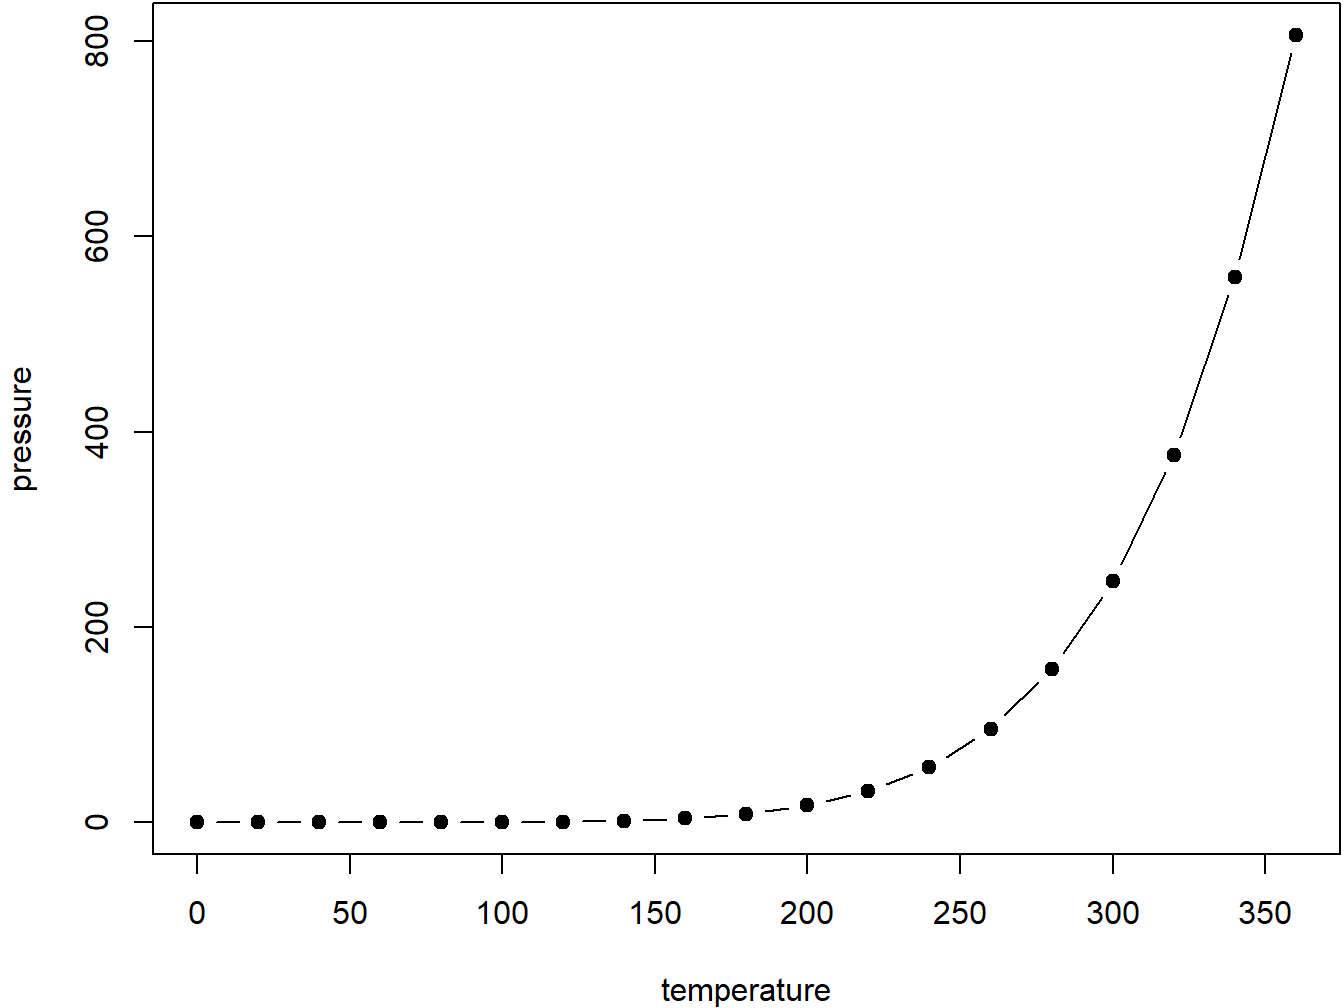
\includegraphics[width=0.8\linewidth]{mystatscourse_files/figure-latex/nice-fig-1} 

}

\caption{Here is a nice figure!}\label{fig:nice-fig}
\end{figure}

Reference a figure by its code chunk label with the \texttt{fig:} prefix, e.g., see Figure \ref{fig:nice-fig}. Similarly, you can reference tables generated from \texttt{knitr::kable()}, e.g., see Table \ref{tab:nice-tab}.

You can also do a text reference for a figure which is useful if you want special characters;



\begin{Shaded}
\begin{Highlighting}[]
\KeywordTok{par}\NormalTok{(}\DataTypeTok{mar =} \KeywordTok{c}\NormalTok{(}\DecValTok{4}\NormalTok{, }\DecValTok{4}\NormalTok{, }\FloatTok{.1}\NormalTok{, }\FloatTok{.1}\NormalTok{))}
\KeywordTok{plot}\NormalTok{(pressure, }\DataTypeTok{type =} \StringTok{'b'}\NormalTok{, }\DataTypeTok{pch =} \DecValTok{19}\NormalTok{, }\DataTypeTok{col=}\DecValTok{2}\NormalTok{)}
\end{Highlighting}
\end{Shaded}

\begin{figure}

{\centering 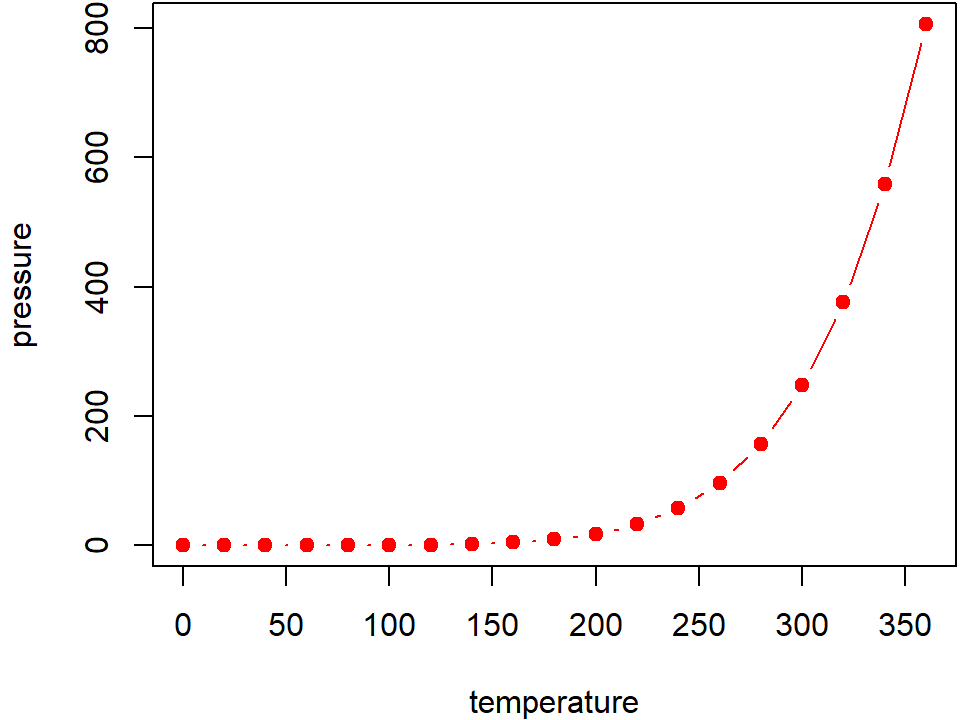
\includegraphics[width=0.8\linewidth]{mystatscourse_files/figure-latex/nice-fig2-1} 

}

\caption{Define a text reference \textbf{here} with some math symbols like \(\theta\).}\label{fig:nice-fig2}
\end{figure}

Here i am referencing \ref{fig:nice-fig2}.

\begin{Shaded}
\begin{Highlighting}[]
\KeywordTok{par}\NormalTok{(}\DataTypeTok{mar =} \KeywordTok{c}\NormalTok{(}\DecValTok{4}\NormalTok{, }\DecValTok{4}\NormalTok{, }\FloatTok{.1}\NormalTok{, }\FloatTok{.1}\NormalTok{))}
\KeywordTok{plot}\NormalTok{(pressure, }\DataTypeTok{pch =} \DecValTok{19}\NormalTok{, }\DataTypeTok{type =} \StringTok{'b'}\NormalTok{)}
\KeywordTok{plot}\NormalTok{(cars, }\DataTypeTok{pch =} \DecValTok{19}\NormalTok{)}
\end{Highlighting}
\end{Shaded}

\begin{center}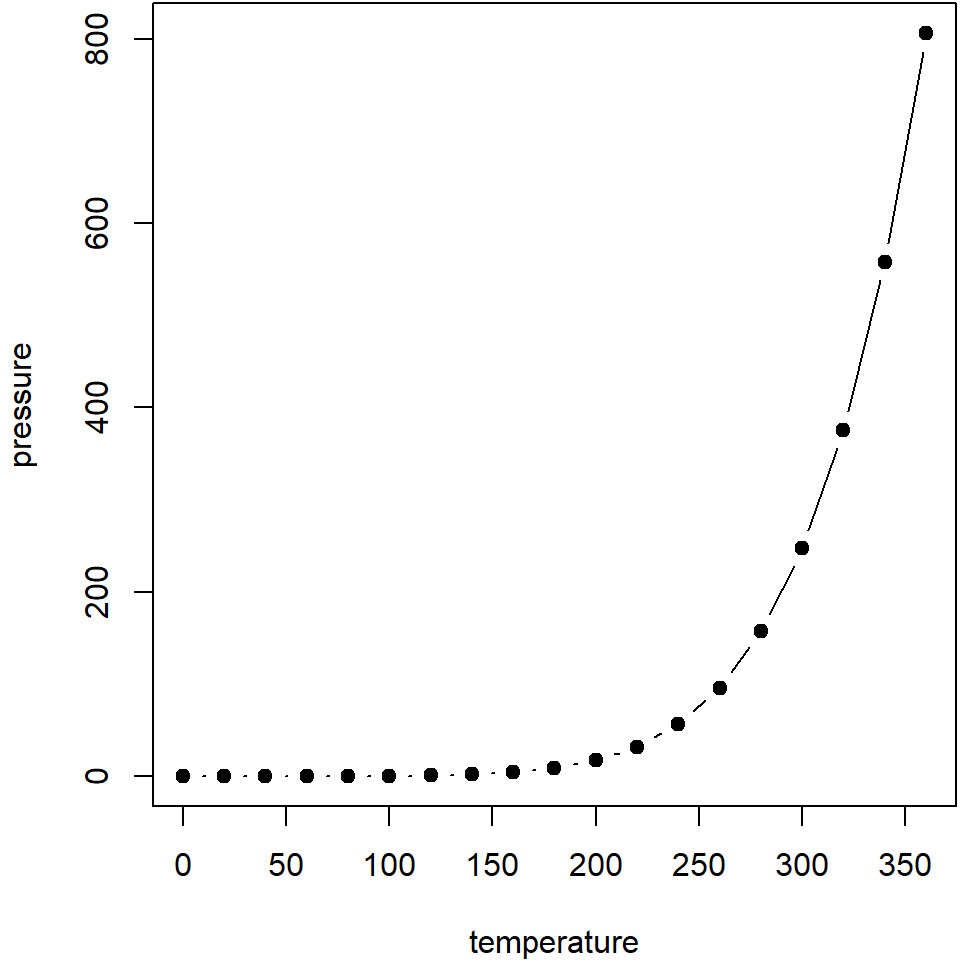
\includegraphics[width=0.5\linewidth]{mystatscourse_files/figure-latex/unnamed-chunk-4-1} 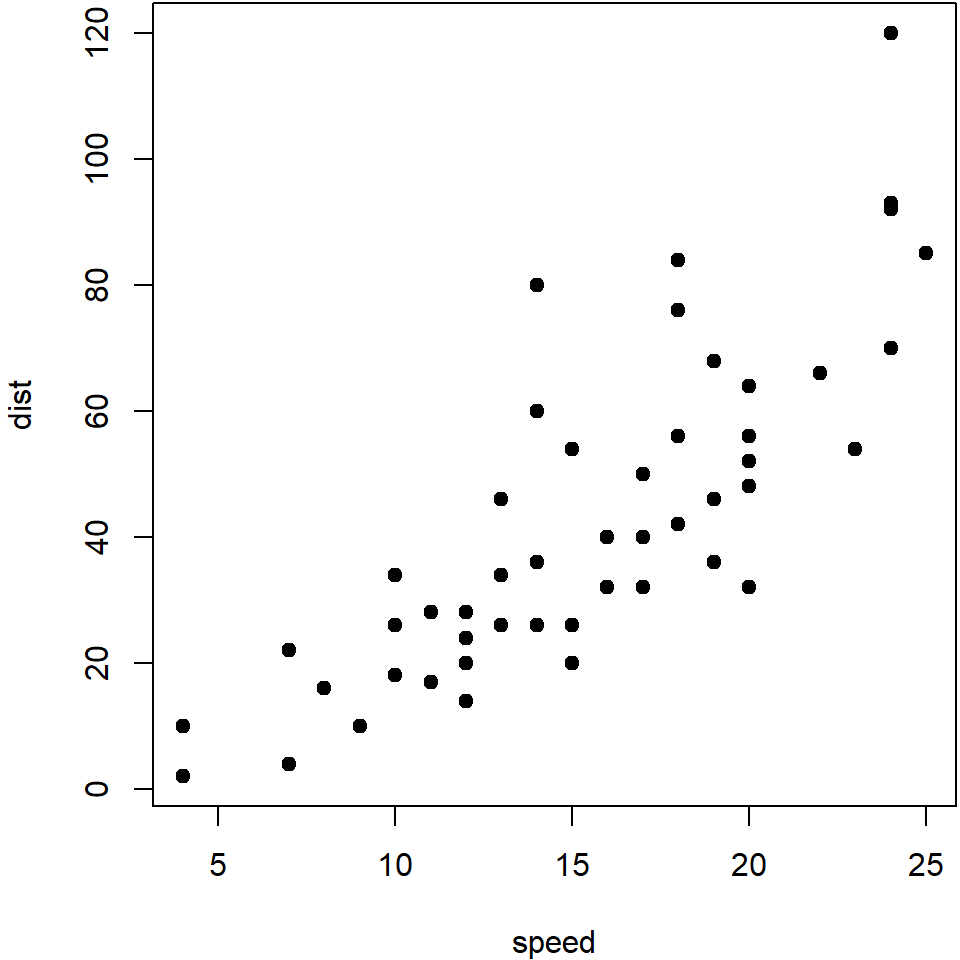
\includegraphics[width=0.5\linewidth]{mystatscourse_files/figure-latex/unnamed-chunk-4-2} \end{center}

\begin{Shaded}
\begin{Highlighting}[]
\NormalTok{knitr}\OperatorTok{::}\KeywordTok{kable}\NormalTok{(}
  \KeywordTok{head}\NormalTok{(iris, }\DecValTok{20}\NormalTok{), }\DataTypeTok{caption =} \StringTok{'Here is a nice table!'}\NormalTok{,}
  \DataTypeTok{booktabs =} \OtherTok{TRUE}
\NormalTok{)}
\end{Highlighting}
\end{Shaded}

\begin{table}

\caption{\label{tab:nice-tab}Here is a nice table!}
\centering
\begin{tabular}[t]{rrrrl}
\toprule
Sepal.Length & Sepal.Width & Petal.Length & Petal.Width & Species\\
\midrule
5.1 & 3.5 & 1.4 & 0.2 & setosa\\
4.9 & 3.0 & 1.4 & 0.2 & setosa\\
4.7 & 3.2 & 1.3 & 0.2 & setosa\\
4.6 & 3.1 & 1.5 & 0.2 & setosa\\
5.0 & 3.6 & 1.4 & 0.2 & setosa\\
\addlinespace
5.4 & 3.9 & 1.7 & 0.4 & setosa\\
4.6 & 3.4 & 1.4 & 0.3 & setosa\\
5.0 & 3.4 & 1.5 & 0.2 & setosa\\
4.4 & 2.9 & 1.4 & 0.2 & setosa\\
4.9 & 3.1 & 1.5 & 0.1 & setosa\\
\addlinespace
5.4 & 3.7 & 1.5 & 0.2 & setosa\\
4.8 & 3.4 & 1.6 & 0.2 & setosa\\
4.8 & 3.0 & 1.4 & 0.1 & setosa\\
4.3 & 3.0 & 1.1 & 0.1 & setosa\\
5.8 & 4.0 & 1.2 & 0.2 & setosa\\
\addlinespace
5.7 & 4.4 & 1.5 & 0.4 & setosa\\
5.4 & 3.9 & 1.3 & 0.4 & setosa\\
5.1 & 3.5 & 1.4 & 0.3 & setosa\\
5.7 & 3.8 & 1.7 & 0.3 & setosa\\
5.1 & 3.8 & 1.5 & 0.3 & setosa\\
\bottomrule
\end{tabular}
\end{table}

Reference this table using Table \ref{tab:nice-tab}

You can write citations, too. For example, we are using the \textbf{bookdown} package \citep{R-bookdown} in this sample book, which was built on top of R Markdown and \textbf{knitr} \citep{xie2015}.

\hypertarget{equations}{%
\section{Equations:}\label{equations}}

\begin{equation} 
  f\left(k\right) = \binom{n}{k} p^k\left(1-p\right)^{n-k}
  \label{eq:binom}
\end{equation}

You may refer to it using \eqref{eq:binom}, e.g., see Equation (2.1).

Please make sure equations \index{equations} without labels are not numbered by either using the equation* environment or adding \nonumber or \notag to your equations. The same rules apply to other math environments, such as eqnarray, gather, align, and so on (e.g., you can use the align* environment).

\begin{align} 
g(X_{n}) & = g(\theta)+g'({\tilde{\theta}})(X_{n}-\theta) \notag \\
\sqrt{n}[g(X_{n})-g(\theta)] & = g'\left({\tilde{\theta}}\right) 
\sqrt{n}[X_{n}-\theta]\label{eq:align} \\
\end{align}

use split to have multiple lines with one equation reference

\begin{equation} 
\begin{split}
\mathrm{Var}(\hat{\beta}) & =\mathrm{Var}((X'X)^{-1}X'y)\\
 & =(X'X)^{-1}X'\mathrm{Var}(y)((X'X)^{-1}X')'\\
 & =(X'X)^{-1}X'\mathrm{Var}(y)X(X'X)^{-1}\\
 & =(X'X)^{-1}X'\sigma^{2}IX(X'X)^{-1}\\
 & =(X'X)^{-1}\sigma^{2}
\end{split}
\label{eq:var-beta}
\end{equation}

there are also `example' and `exercise' environments (labelled with exm and exr respectively)

\begin{example}[how to do an example]
\protect\hypertarget{exm:eg1}{}{\label{exm:eg1} \iffalse (how to do an example) \fi{} }for this example, we show nothing
\end{example}

\begin{example}[how to do a second example]
\protect\hypertarget{exm:eg2}{}{\label{exm:eg2} \iffalse (how to do a second example) \fi{} }for this example, we show something
\end{example}

these environments can be changed using the css file
CSS class being the environment name, e.g., \texttt{\textless{}div\ class="lemma"\textgreater{}\textless{}/div\textgreater{}}

\hypertarget{literature}{%
\chapter{Literature}\label{literature}}

Here is a review of existing methods.

\hypertarget{methods}{%
\chapter{Methods}\label{methods}}

We describe our methods in this chapter.

We showed some examples in the introduction (Chapter \ref{intro})

You can also reference specific sections by giving them a label \texttt{\{\#sectionname\}}

And you can add words to the index such as GLM \index{GLM}

\hypertarget{shiny-app}{%
\section{Shiny app}\label{shiny-app}}

\hypertarget{type-1---calling-from-shinyapps.io}{%
\subsection{type 1 - calling from shinyapps.io}\label{type-1---calling-from-shinyapps.io}}

\begin{figure}

{\centering \href{https://lindesaysh.shinyapps.io/mt1007_week22/}{\includegraphics{mystatscourse_files/figure-latex/myshiny-1} }

}

\caption{An eaxmple of a shiny app. you can see a live version at (put url here)}\label{fig:myshiny}
\end{figure}

you can use a shiny app embedded in the notes Figure \ref{fig:myshiny}.

\hypertarget{type-3---creating-inline}{%
\subsection{type 3 - creating inline}\label{type-3---creating-inline}}

\hypertarget{applications}{%
\chapter{Applications}\label{applications}}

\begin{Shaded}
\begin{Highlighting}[]
\KeywordTok{library}\NormalTok{(ggplot2)}
\end{Highlighting}
\end{Shaded}

Some \emph{significant} applications are demonstrated in this chapter.

\hypertarget{example-one}{%
\section{Example one}\label{example-one}}

\hypertarget{example-two}{%
\section{Example two}\label{example-two}}

\begin{quote}
\textbf{Aside}: using the model to predict outside of the range of the observed data is called \textbf{extrapolating}. Oftentimes, statistical models are developed \emph{in order} to be used to extrapolate (e.g.~climate modelling). This is however, dangerous, as we can only assess the assumptions of the model over the range of the observed data. When extrapolating we have to assume that these relationships hold beyond the range of the data, which may or may not be reasonable (hence why weather forecast over short-time periods are OK, but climate forecasts are much more uncertain). Hence, we should always view the model as an approximation of the data generating process. In this particualr case, the interpretation of the parameters is not sensible when \(x = 0\) (weight = 0 kg), but makes sense in the range that we are interested in exploring. If the case where \(x = 0\) is important, then we would have to change the model to ensure that the predictions made sense at those values of \(x\).
\end{quote}

\hypertarget{tsk1}{}\bblockT[Task]{\phantomsection\label{sol1}1}

Produce a scatterplot of \texttt{mpg} against \texttt{hp}. What does the relationship look like?

\eblockT

\hyperlink{sol1}{\buttonS{Show Solution on P\colpageref{tsk1}}}

\hypertarget{final-words}{%
\chapter{Final Words}\label{final-words}}

We have finished a nice book.

If you want to split the book by sections, so each html page is a section you can use split\_by=`section' in the YAML header.

\begin{verbatim}
output: 
   bookdown::gitbook:
    lib_dir: "book_assets"
    config:
      sharing: null
    split_by: section
\end{verbatim}

\hypertarget{appendix-appendix}{%
\appendix}


\hypertarget{answers}{%
\chapter{Answers}\label{answers}}

\hypertarget{sol1}{}
\bblockS[Solution]{\phantomsection\label{tsk1}1}

\begin{Shaded}
\begin{Highlighting}[]
\KeywordTok{plot}\NormalTok{(hp }\OperatorTok{~}\StringTok{ }\NormalTok{mpg, }\DataTypeTok{data =}\NormalTok{ mtcars, }
  \DataTypeTok{pch=}\DecValTok{19}\NormalTok{, }\DataTypeTok{col=}\StringTok{'darkgrey'}\NormalTok{)}
\end{Highlighting}
\end{Shaded}

\begin{center}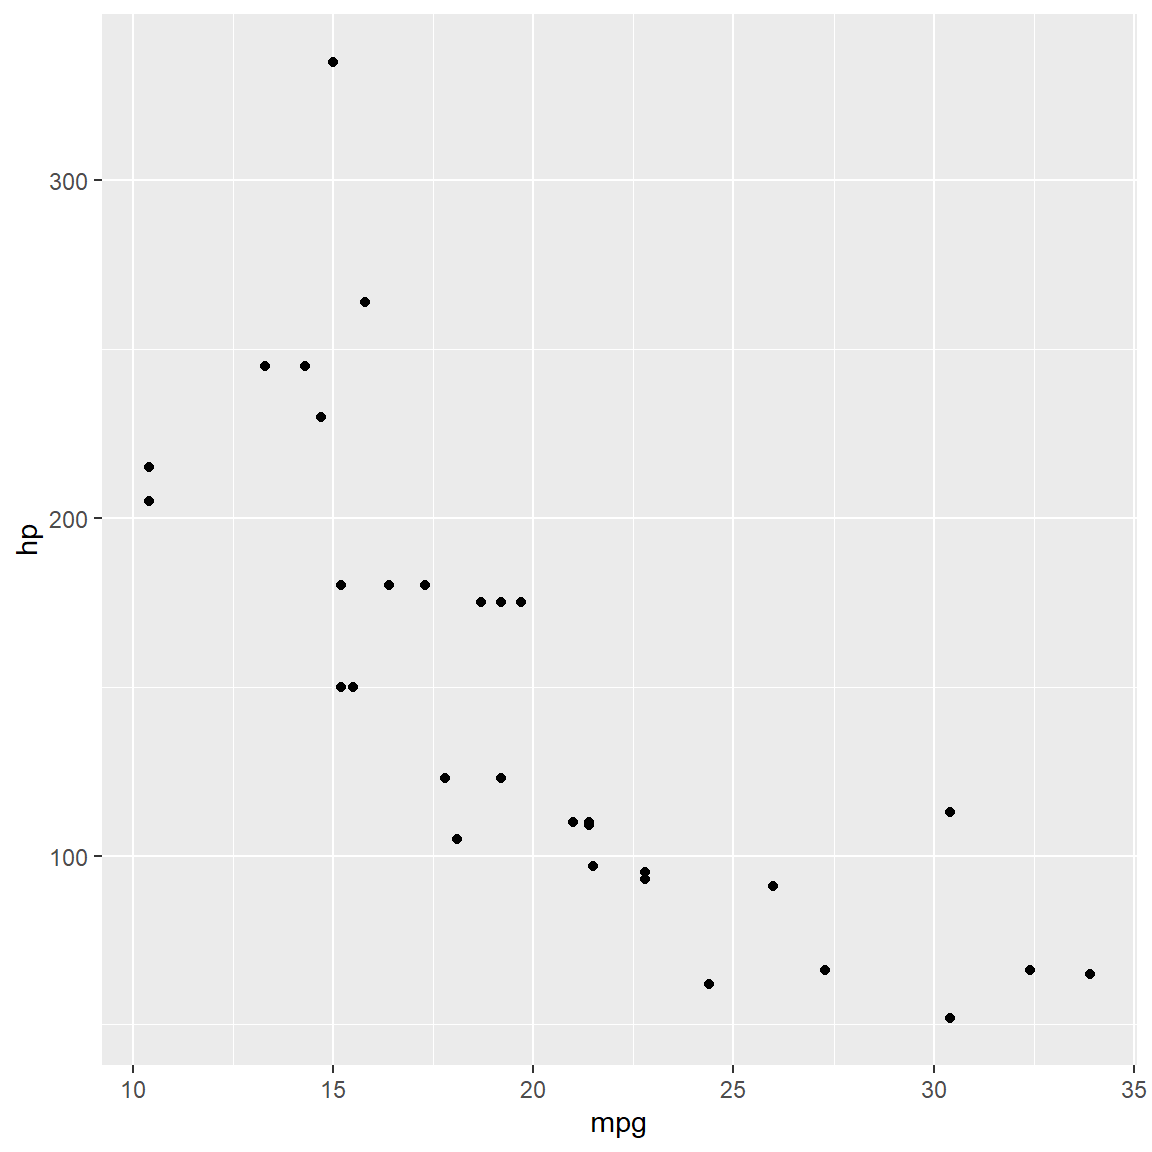
\includegraphics{mystatscourse_files/figure-latex/unnamed-chunk-10-1} \end{center}

This is my solution

\vspace{\baselineskip}

\hyperlink{tsk1}{\buttonT{Return to task on P\colpageref{sol1}}}
\eblockS

  \bibliography{book.bib,packages.bib}

\printindex

\end{document}
